% ----------------------------------------------------------
\chapter{Experiments and Results}\label{ch:experiments}
% ----------------------------------------------------------

In this chapter, we build on the theoretical foundations exposed above and propose a novel solution method for \glspl{IVP} of \glspl{ODE}.
The main goal of the chapter is to validate the approach and explore its performance under different hyperparameter configurations.
This is done through a series of experiments on the Van der Pol oscillator.

We benchmark our approach to \glspl{PINN}, a well-established deep learning solution to this kind of problem.
The comparison is made both in terms of approximation error and in solution speed.
Overall, this chapter lays out the results for the discussion provided in Chapter \ref{ch:conclusion}.

\section{Problem Definition}

The Van der Pol oscillator (Sec. \ref{sec:vdp}) was chosen as the \gls{ODE} system for which an \gls{IVP} will be solved.
This system is known for having no analytical solution, thus becoming a benchmark for solvers.
As well, \textcite{Antonelo2021} have already studied a solution using \gls{PINN}s, which is considered as a starting point and a reference for performance in the experiments.

More specifically, we define the first-order formulation of the Van der Pol oscillator (as presented in Equation \eqref{eq:vdp}) as the \gls{ODE} system, with $\mu=1$.
Then, the \gls{IVP} is defined with initial condition $\bm{y}(0) = \bm{y}_0 = \left( 0, 0.1 \right) $, simulating a small perturbation to the system around the unstable equilibrium at the origin. The solution is desired for a horizon of 2 seconds. 
In this interval, the solution is expected to gravitate to a limit cycle, as illustrated in Figure \ref{fig:vdp_example}.

\subsection{Evaluation Metrics}

As there is no analytical solution to the \gls{IVP} at hand, the solutions will be evaluated in comparison to the approximation found using \gls{RK4}.
This reference was generated from 1000 points equally spaced in the solution interval $I=[0,2]$, with a time step of 2\,ms\footnotemark.
\footnotetext{Of course, this set does not include the initial condition, which is already given, meaning that the first point of evaluation is at $t=0.002$.}
Then, a solution's approximation to the reference is measured through the \gls{IAE}, which can be defined here as \[
    IAE = \frac{1}{h}\sum_{i=1}^{1000} \|\bm{y}_i - \hat{\bm{y}}_i\|
,\] where $\bm{y}_i$ are the points in the \gls{RK4} solution,  $\hat{\bm{y}}_i$ are the points in the solution being evaluated, and $h=0.002$ is the time step.
Therefore, a solution is said to be suitable for the problem if it achieves a low \gls{IAE}.

Besides the quality of the approximation, the time required to achieve such an approximation is also of interest, as many applications (e.g., model predictive control) are highly time-dependent.
The hardware resources used are valuable metrics, as the necessary computing power limits the range of equipment that can support a given solution.
These will be auxiliary to the \gls{IAE} in the analysis of the approximations.

\section{PIDEQ}\label{sec:pideq}

As already discussed in Section \ref{sec:pinn-problem}, solving \gls{IVP}s is (mostly) only reasonable if using a physics-informed approach, that is, if ``teaching'' the model through the known dynamics instead of through actual samples of the target function.
Therefore, a reasonable solution using \gls{DEQ}s must follow the same principle, which implies in a physics-informed training of \gls{DEQ}s (thus the naming \gls{PIDEQ}).

For the \gls{IVP} defined above, we recall the definition of Section \ref{sec:deq-definition} and propose a \gls{DEQ} similar to \textcite{Ghaoui2019}, that is, a model
\begin{align*}
    D_{\gls{param}}^{EQ}: \R &\longrightarrow \R^2 \\
    t &\longmapsto D_{\gls{param}}(t) = \hat{\bm{y}}
\end{align*}
such that
\begin{equation}
\begin{split}
    D^{EQ}_{\gls{param}}(t) &= C\bm{z}^{\star} \\
    \bm{z}^{\star} &= \bm{f}_{\gls{param}}\left( t,\bm{z}^{\star} \right) \\
    \bm{f}_{\gls{param}}\left( t,\bm{z} \right) &= \tanh \left( A\bm{z} + t\bm{a} + \bm{b} \right)
\end{split}
,\end{equation}
in which the parameters \gls{param} are a vectorization of the matrices and vectors, i.e., $\gls{param} = \left( A,C,\bm{a},\bm{b} \right)$, and the hyperbolic tangent function is applied to each element of the resulting vector.

Notice that this formulation is very close to the one used in Chapter \ref{ch:deq}, except for the linear transformation of the equilibrium point at the model's output.
This implies that both forward and backward operations can occur in the same way, except that the term  \[
    \frac{d D^{EQ}_{\gls{param}}}{d \bm{z}^{\star}} = C
\] must be considered in the computation of the gradients.
The advantage of this modification is that we can have $\bm{z}$ with an arbitrary dimension, that is, we can have an arbitrary \emph{number of states}, which results in arbitrary representational power \cite{Ghaoui2019}.

The challenge in physics-informing a \gls{DEQ} is to optimize a cost function on its derivatives.
As it was shown in Section \ref{sec:deq-backward}, \textcite{Bai2019} have proposed an efficient way to compute the first derivative of a \gls{DEQ} with regard to either its parameters or the input, which allows us to compute the cost function value.
Yet, for an application of gradient descent with such cost function, it is required that the second derivatives of the model (with respect to the input and the parameters) are computable during training time.
In practice, this implies in the computation of the derivative of the root-finding algorithm used to compute the first derivative, as seen in Section \ref{sec:deq-backward-implementation}.\footnotemark
\footnotetext{In theory, it could be possible to use the implicit function theorem once again to achieve an analytical formula for the second derivative, but this is left for future work.}
This restricts us to using differentiable root-finding algorithms to compute the first derivative, relying on automatic differentiation tools to compute the second derivative.

Finally, we propose to use a cost function for training a \gls{PIDEQ} model of the form \[
    J\left( \gls{param} \right) = J_b\left( \gls{param} \right) + \lambda J_{\mathcal{N}}\left( \gls{param} \right) + \kappa \left\lVert \frac{d \bm{f}_{\gls{param}}}{d \bm{z}}\right\rVert_F
,\] 
in which $J_b$, $J_{\mathcal{N}}$ and $\lambda$ are as defined in Section \ref{sec:PI}, while $\left\lVert \frac{d \bm{f}_{\gls{param}}}{d \bm{z}}\right\rVert_F$ is the Frobenius norm of the Jacobian of the equilibrium function, as exposed in Sec. \ref{sec:deq-jac-reg}, a regularization term weighted by $\kappa \in \R_+$.
This cost function ensures the physics-informed training from \gls{PINN}s with the regularization term which was shown essential to \gls{DEQ}s.

\section{Training}

Early experiments helped to define the design choices for the training algorithm and the hyperparameters.
Adam~\cite{kingma_adam_2015} was the optimizer of choice, with $\gls{lr}=0.001$ and default configuration.
The cost-weighting coefficients were initially set as $\lambda=0.1$ and $\kappa=1.0$.
The solver used for the forward pass of the model was the Anderson Acceleration~\cite{walker_anderson_2011}, while best results were found using simple iteration to compute the backward pass.
% \footnotetext{More complex solvers, even if made differentiable for the automatic differentiability package, had such an increased cost for computing the second derivative that the simple iteration became a much better choice.}
For both algorithms, the tolerance was set as $\varepsilon=10^{-4}$ and they were limited to 200 iterations.
The initial guess was always $\bm{z}_0=\bm{0}$.

The set $X_b$, of course, contained only the initial condition, while $X_{\mathcal{N}}$ contained $10^5$ random samples within $I$.
The regularization term $\left\lVert \frac{d \bm{f}_{\gls{param}}}{d \bm{z}}\right\rVert_F$ was computed on the input values of both data sets.

\section{Experiments}

The experiments reported below concern the training of the deep learning model proposed above to solve the \gls{IVP} described in the first section of this chapter.
The implementation was done using PyTorch \cite{paszke_pytorch_2019} and is available at \url{https://github.com/brunompacheco/pideq}.
All experiments were performed on a high-end computer, using an RTX 3060 GPU.
A budget of 50000 epochs was chosen.
5 models with each configuration were trained, with different initial (random) weights.

\subsection{Baseline Results}

The baseline result for a \gls{PINN} trained to solve an \gls{IVP} of the Van der Pol oscillator comes from \textcite{Antonelo2021}.
We replicate these results, that is, a traditional \gls{PINN} with 4 hidden layers with 20 nodes each, following the same setup proposed above (except for the regularization term of the cost function).
At the same time, \textcite{Ghaoui2019} showed that a \gls{DEQ} with as many states as there are hidden nodes in a given deep feedforward network, has \emph{at least} as much representational power as that network.
Then, our starting \gls{DEQ} is a model with 80 states.
The results for both models can be seen in Figure \ref{fig:baseline-iae}.

\begin{figure}[h]
    \centering
	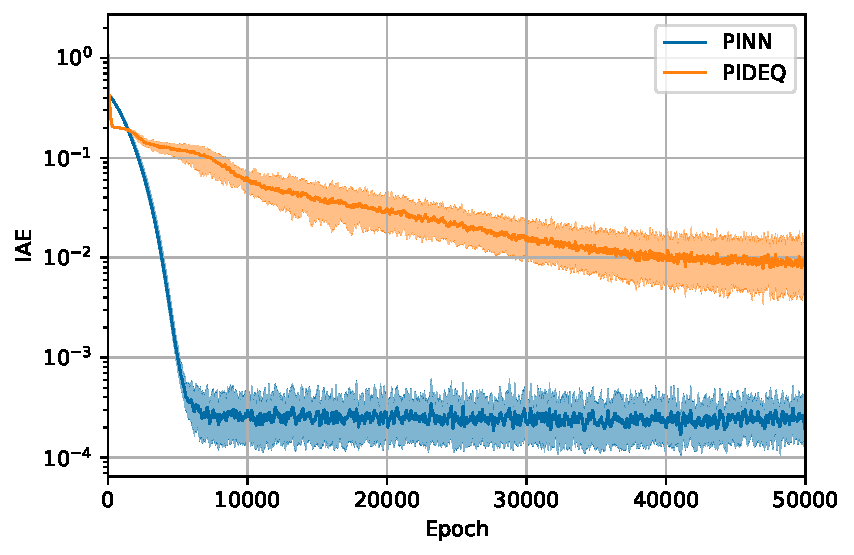
\includegraphics{images/exp_1_iae.pdf}
    \caption{Learning curve for the baseline models trained on the \gls{IVP} for the Van der Pol oscillator. Solid lines are mean values ($n=5$), shaded regions represent minimum and maximum values. For a better visualization, a moving average of 100 epochs was taken.}
    \label{fig:baseline-iae}
\end{figure}

Given that the \gls{PINN} was able to ``learn'' (i.e., to achieve a low IAE on) the task, we expect that the large \gls{PIDEQ} model also is capable of learning.
\glspl{PIDEQ} indeed achieved a low IAE, yet not as low as the \glspl{PINN}.
Furthermore, \glspl{PIDEQ} had a much slower convergence rate, while \glspl{PINN} converged in under 10000 epochs.
Besides being much more complex (in its structure) than the feedforward network, the \gls{PIDEQ} also has many more parameters, in a total of 6802 against 1342.
This results in a big difference in the effective training time: the \gls{PINN}s took, on average, 11\,ms for each epoch, while the \gls{PIDEQ}s took 209\,ms.

\subsection{Number of States}

A deeper look at the $A$ matrix of the baseline \gls{PIDEQ}s after training, as illustrated in Figure \ref{fig:baseline-pideq-A}, shows that many of the rows are practically zero vectors, in comparison to the remaining.
Having ``empty'' rows implies that the states associated with these rows are not effectively contributing to the results, that is, given the parameters of this model, a smaller model could be constructed with the same result.  

\begin{figure}[h]
    \centering
    \begin{subfigure}[t]{.45\textwidth}
	\vspace{0pt}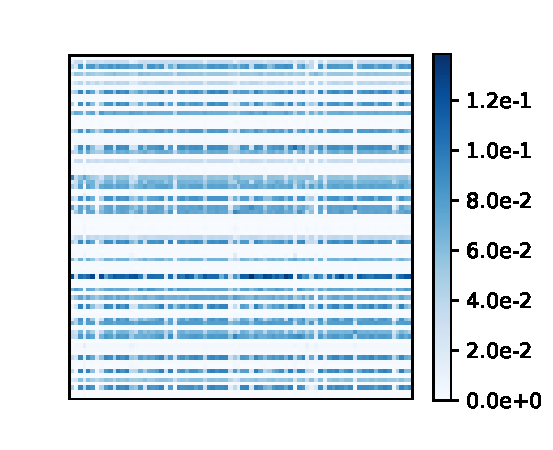
\includegraphics{images/exp_1_matplot.pdf}
	\caption{Magnitude of the elements of $A$. White is 0.}
    \end{subfigure}
    \begin{subfigure}[t]{.45\textwidth}
	\vspace{0pt}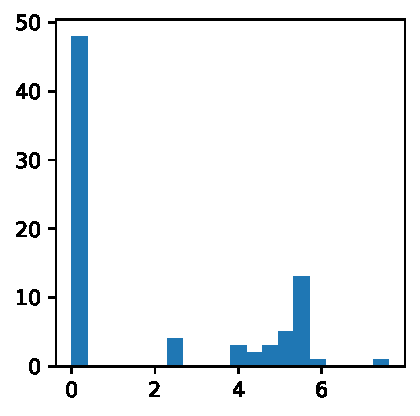
\includegraphics{images/exp_1_hist.pdf}
	\caption{Histogram of $\ell_1$ norm of the rows of $A$.}
    \end{subfigure}
    \caption{$A$ matrix of the baseline \gls{PIDEQ} after training. From all models trained, the one with median final performance was used to generate the graphics.}
    \label{fig:baseline-pideq-A}
\end{figure}

This analysis motivates the training of models with fewer states.
The experiment was defined as an iterative procedure based on the intuition above.
A new model was trained with fewer states, its $A$ matrix was analyzed, and, if there were still empty rows in the $A$ matrix, a new model was proposed with even fewer states.
This procedure was repeated for models with 40, 20, 10 and 5 states.
The models with 5 states showed no ``empty rows'' in the $A$ matrix, as shown in Figure \ref{fig:mat-pideq-5}, but still a model with only two states was trained.
The results can be seen in Figure \ref{fig:states-iae}.

\begin{figure}[h]
    \centering
    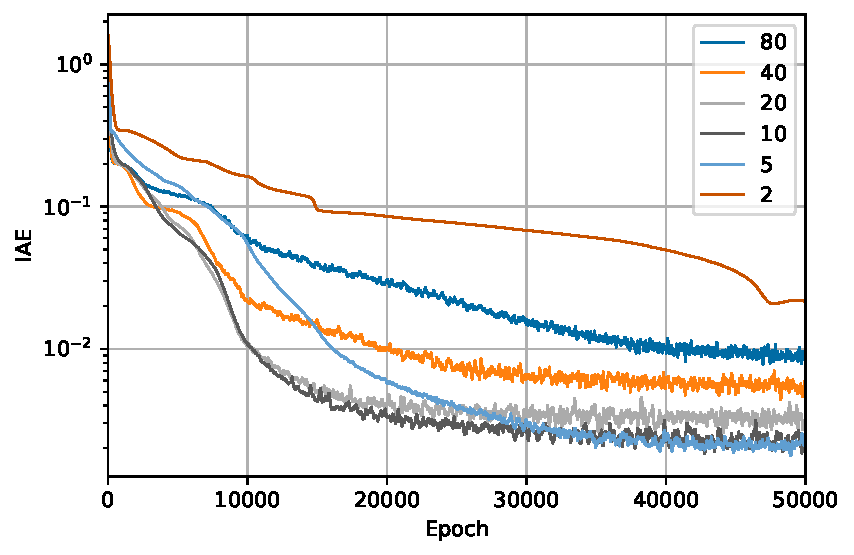
\includegraphics{images/exp_2_iae.pdf}
    \caption{Learning curve of the models trained with fewer states. Solid lines are mean values ($n=5$). For a better visualization, a moving average of 100 epochs was taken.}
    \label{fig:states-iae}
\end{figure}

\begin{figure}[h]
    \centering
    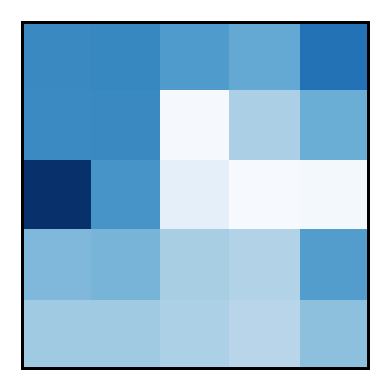
\includegraphics{images/exp_2_matplot.pdf}
    \caption{$A$ matrix of the \gls{PIDEQ} with 5 states. From the 5 models trained, the one with median final performance was selected to generate the graphic.}
    \label{fig:mat-pideq-5}
\end{figure}

The smaller models achieve even better results than the baseline and converge much faster, except for the smallest one, which was not able to learn within the training budget, reinforcing the intuition exposed above.
The model with 5 states takes more epochs to converge, intuitively this can be attributed to it being close to its representational limit, but as it is much smaller (with only 52 parameters), it trains faster than the larger ones.
Table \ref{tab:n-states-times} exposes the times for each model.

\begin{table}[h]
    \centering
    \caption{Median training and validation times per epoch for \gls{PIDEQ} models with different number of states.}
    \label{tab:n-states-times}
    \begin{tabular}{ccc}
	\toprule
	\textbf{Number of States} & \textbf{Train} [ms] & \textbf{Validation} [ms] \\ \midrule
	80       & 99.1       & 2.1             \\
	40       & 51.2       & 1.7             \\
	20       & 37.1       & 1.2             \\
	10       & 29.7       & 1.1             \\
	5        & 26.0       & 1.2             \\
	2        & 24.8       & 1.2             \\ \bottomrule
    \end{tabular}
\end{table}

\subsection{Jacobian Regularization}\label{sec:exp-jac}

Following the previous results, the impact of the Jacobian regularization term in the cost function is explored for the model with 5 states.
From the work of \textcite{bai_stabilizing_2021}, it is expected that this regularization term will have an impact on the results.
We verify this by training \gls{PIDEQ} models without such term ($\kappa=0$) and with a reduced importance ($\kappa=0.1$).
The results are shown in Figure \ref{fig:jac-lamb-iae}.

\begin{figure}[h]
    \centering
    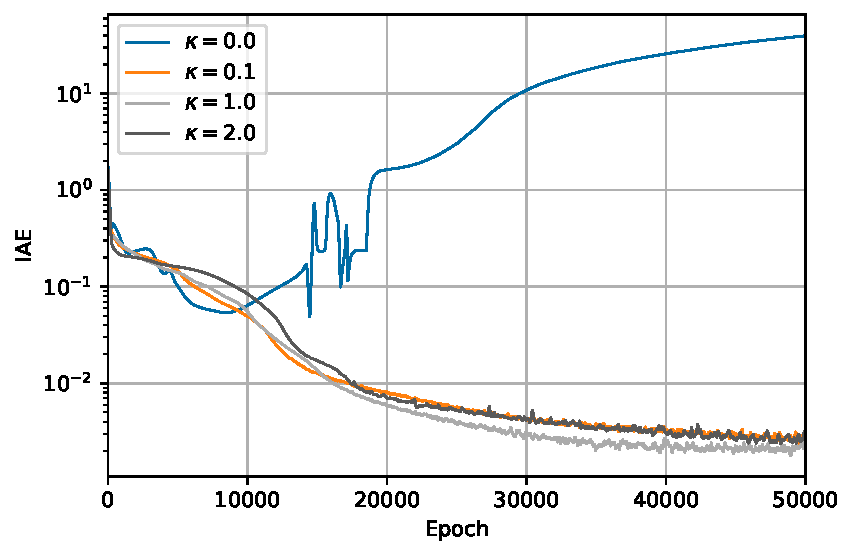
\includegraphics{images/exp_4_iae.pdf}
    \caption{Learning curve for \gls{PIDEQ}s with different $\kappa$ values. Only one model was trained with $\kappa=0$ because the training took over 30 times longer. Solid lines are mean values ($n=5$). For a better visualization, a moving average of 100 epochs was taken.}
    \label{fig:jac-lamb-iae}
\end{figure}

The experiments confirm the theory in that training without the regularization was ineffective.
Not using the regularization term resulted in models not learning the task and taking over 30 times longer to train.
At the same time, increasing or decreasing the impact of the regularization term in the cost function resulted in worse models overall.

\subsection{Solver}

As discussed in Section \ref{sec:pideq}, the solver used within the computation of the first derivative of \glspl{PIDEQ} must be differentiable, and, for the experiments, was fixed as the simple iteration method.
Nevertheless, the impact of the solver used for the forward pass can be explored.
Since the derivative is computed implicitly, solver's impact in the inference and training speed is clearer.
Yet, as the algorithm of different solvers define different paths through the domain to find an equilibrium point, different equilibria can be found given distinct solvers, which can change the performance of the model with respect to error levels. 

In fact, this behavior is observed in the results of the experiments comparing Anderson's Acceleration with simple iteration and Broyden's method~\cite{broyden_class_1965} for the forward pass, as seen in Figure \ref{fig:solver-iae}.
Models using Broyden's method achieve a smaller error, but the iterations took much longer, with a median value of 212 ms in comparison to 27 ms using Anderson Acceleration.
At the same time, using simple iteration resulted in a performance as good as using Anderson Acceleration, but with a median epoch time of 9 ms.
Of course, as was discussed in Section \ref{sec:deq-forward}, simple iteration is less reliable than the other two methods, yet, it seems to work well for the problem at hand.

\begin{figure}[h]
    \centering
    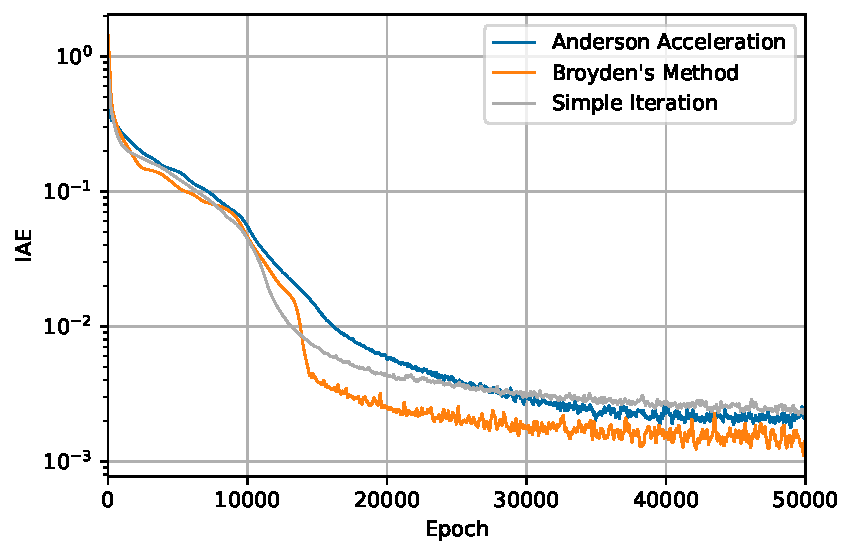
\includegraphics{images/exp_5_iae.pdf}
    \caption{Learning curve of \gls{PIDEQ} models with 5 states using different solvers for the forward pass. Solid lines are mean values ($n=5$). For a better visualization, a moving average of 100 epochs was taken.}
    \label{fig:solver-iae}
\end{figure}

\subsection{Solver Tolerance}

As the previous experiment showed, the simple iteration was the best approach, given the trade-off between prediction quality and training speed.
Then, the $\varepsilon$ parameter is explored next.
Intuitively, it is expected that a smaller tolerance imply in a slower training but a smaller error.
The results with models trained using the simple iteration algorithm with $\varepsilon \in \left[ 10^{-2}, 10^{-4},10^{-6} \right] $, as exposed in Figure \ref{fig:epsilon-iae}, confirm that the tolerance is indeed impactful, as increasing the "default" tolerance (of $10^{-4}$) tends to increase the error of the trained models.
At the same time, a decreased tolerance did not improve the performance within the training budget, possibly pointing that the default value is already sufficient for the problem.

\begin{figure}[h]
    \centering
    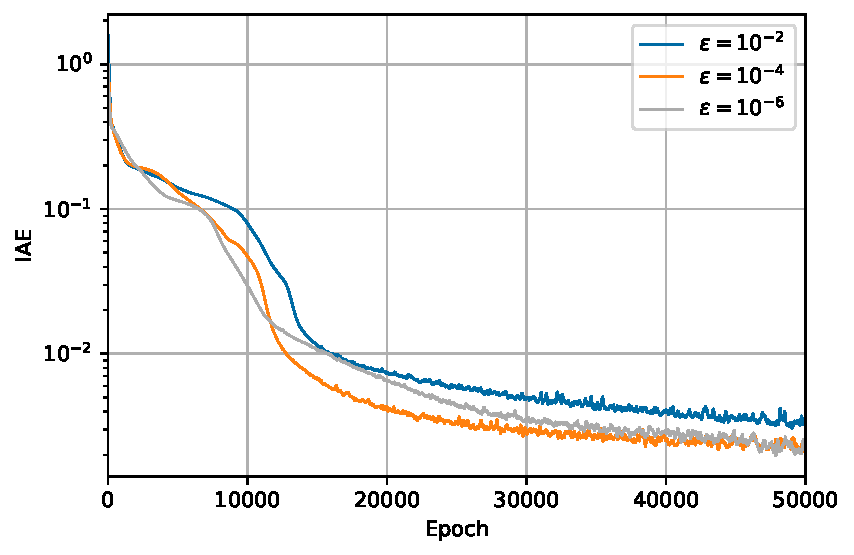
\includegraphics{images/exp_6_iae.pdf}
    \caption{Learning curve of \gls{PIDEQ} models with 5 states when trained with different tolerances for the simple iteration solver. Solid lines are mean values ($n=5$). For a better visualization, a moving average of 100 epochs was taken.}
    \label{fig:epsilon-iae}
\end{figure}

\subsection{Final Model}

The previous experiments showed how a much smaller a model can be used together with the simple iteration method, which provides a faster training.
In comparison to the initial \gls{PIDEQ}, there was a significant decrease in the error.
Yet, the biggest impact was in training time, which decreased from 99 ms to 9 ms for each epoch (median value). 
The \gls{PIDEQ} with only 5 states also has significantly fewer parameters (52), since the number of parameters grows quadratically with the number of states.
A reduced number of parameters implies in less memory consumption and in greater explainability.

For a fair comparison, \gls{PINN} models were trained with only 52 parameters, i.e., with only two hidden layers, each with dimension 5.
The performance of the final model and the small \gls{PINN} model can be assessed in Figure \ref{fig:final-iae}, in comparison to the baseline models. The final models can be assessed visually, against \gls{RK4}'s approximate solution, through the graphics in Figure \ref{fig:final-vdp}.

\begin{figure}[h]
    \centering
    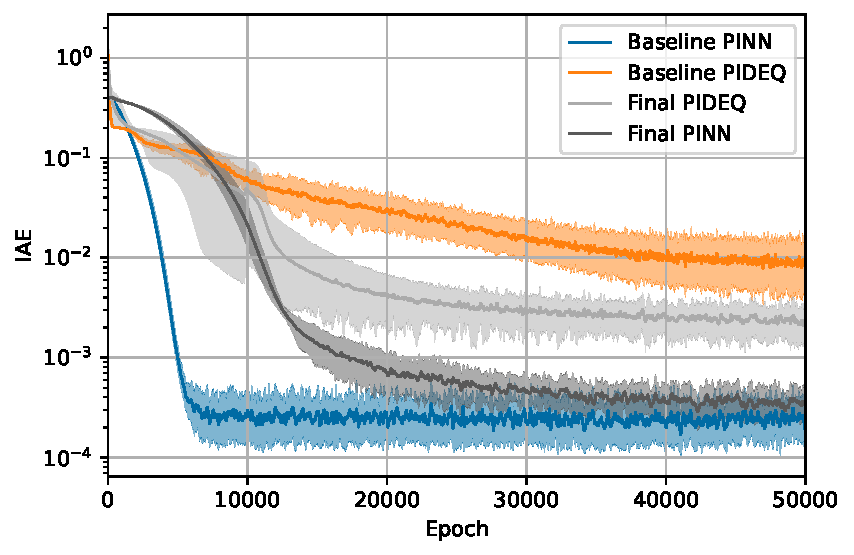
\includegraphics{images/final_iae.pdf}
    \caption{Learning curve of the final models in comparison to the baselines. ``Final PINN'' are the small \gls{PINN} models, with only 52 parameters. ``Final PIDEQ'' are the \gls{PIDEQ} models with 5 states and using the simple iteration method as solver for the forward pass. Solid lines are mean values ($n=5$), shaded regions represent minimum and maximum values. For a better visualization, a moving average of 100 epochs was taken.}
    \label{fig:final-iae}
\end{figure}

\begin{figure}[h]
    \centering
    \begin{subfigure}[t]{.45\textwidth}
	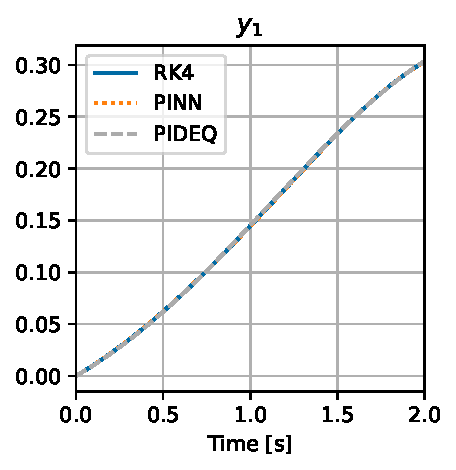
\includegraphics{images/final_vdp_y1.pdf}
	\caption{}
    \end{subfigure}
    \begin{subfigure}[t]{.45\textwidth}
	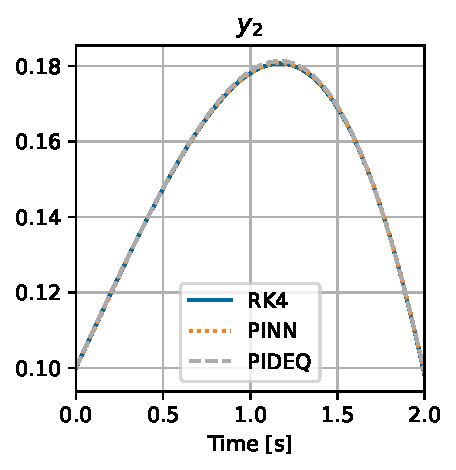
\includegraphics{images/final_vdp_y2.pdf}
	\caption{}
    \end{subfigure}
    \caption{Prediction of \gls{PINN} and \gls{PIDEQ} in comparison to the reference approximation resulting from \gls{RK4}. Both models presented the median performance in the respective experiments.}
    \label{fig:final-vdp}
\end{figure}

Both final models take around the same number of epochs to converge, but the \gls{PINN} models are able to achieve much smaller errors, almost as low as the baseline models.
The small \glspl{PINN} also have a smaller training time.
A breakdown of the time per epoch spent by each approach can be seen in Figure \ref{fig:final-times}.
As expected, \glspl{PIDEQ} take longer to compute the output, which is a direct implication of computing the equilibrium and storing intermediate values to compute the derivatives.
This, however, does not translate to inference, as both approaches take approximately the same to compute the validation results each epoch.
Computing the total cost is a more expensive operation for \glspl{PIDEQ}.
This extra cost comes mostly from the regularization term necessary to convergence, as seen in the experiments from Section \ref{sec:exp-jac}.
It is surprising, however, how the \glspl{PIDEQ} did not take longer than \gls{PINN} models to back-propagate the cost and update the parameters..

\begin{figure}[h]
    \centering
    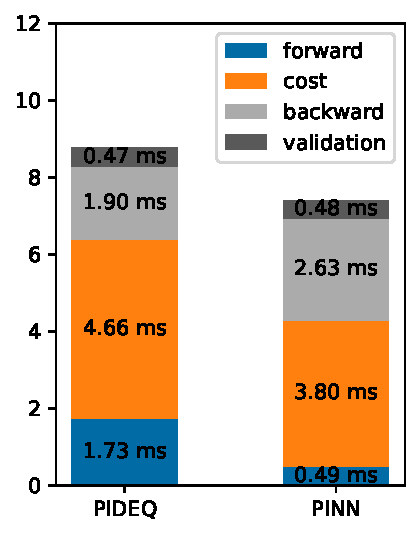
\includegraphics{images/final_times.pdf}
    \caption{Breakdown of median time per epoch for the final \gls{PIDEQ} and the small \gls{PINN}. ``forward'' represents the time necessary to compute the output given the input during the training time (with gradients computation enable). ``cost'' indicates the time necessary to compute the cost function, given the predictions. ``backwards'' is the time necessary to back-propagate the cost to the parameters.}
    \label{fig:final-times}
\end{figure}

